% B / onlysonder：跨重复验证，放在候选发现之后。
\begin{frame}{在 WT 另一重复中核查候选}
\textbf{每个独立位置，固定一个 rep1 代表窗口与 rep2 比较。}
\vspace{0.8em}
\begin{columns}[T,onlytextwidth]
\begin{column}{0.47\textwidth}
\textcolor{projectblue}{\large\textbf{10 个代表窗口}}\par\vspace{0.6em}
Pearson $r=0.664$--$0.916$\par
中位数：\textbf{0.857}\par\vspace{0.6em}
4 个窗口含数据缺口，相关仅在共同有效区域计算。
\end{column}
\begin{column}{0.47\textwidth}
\textcolor{projectblue}{\large\textbf{与已知注释的关系}}\par\vspace{0.6em}
8 个位置与已知结构重叠。\par\vspace{0.5em}
去重命中：OPCID 10、CHIN 10、CHID 1，共 21/344。\par\vspace{0.5em}
2 个未重叠位置未满足新簇条件。
\end{column}
\end{columns}
\vspace{1em}
\small 比较采用同坐标 O/E 和共同有效上三角；结果支持代表窗口的图形一致性。
\end{frame}

\begin{frame}{候选 035：两个重复的接触图形}
\centering
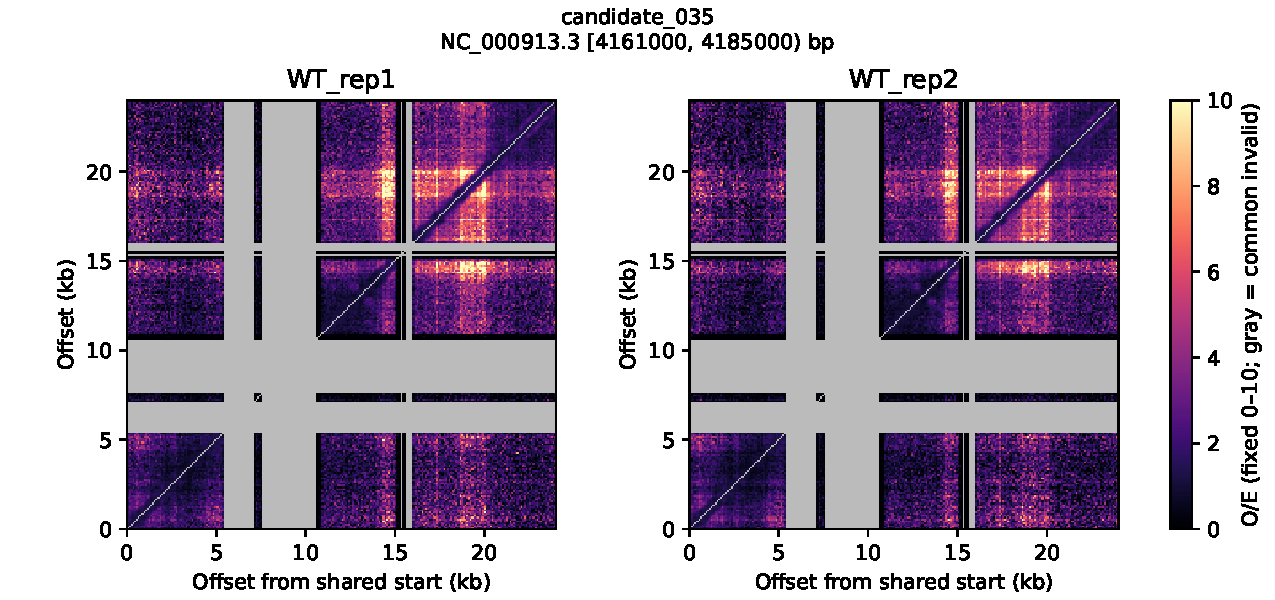
\includegraphics[width=0.90\textwidth,height=0.59\textheight,keepaspectratio]{../results/validation/paired_oe/candidate_035.pdf}\par
\vspace{0.6em}
\raggedright\small
共同有效上三角像素 \textbf{17,578}（61.29\%），Pearson $r=\textbf{0.7402}$。\par
两图共用坐标、mask 和色标；灰色缺口排除在计算之外。
\end{frame}
